Τα σχήματα \ref{fig:02_02_04:selections_orientation_zoomed} και
\ref{fig:02_02_04:selections_position_zoomed} δείχνουν την κατανομή όλων των
σφαλμάτων εκτίμησης προσανατολισμού και θέσης, αντίστοιχα, των μεθόδων επιλογής
σωματιδίων από τον πληθυσμό του MCL για την ελάττωση του σφάλματος εκτίμησής
του.

\begin{figure}
  \vspace{2cm}
  \begin{subfigure}{\linewidth}
  \hspace{-1.25cm}
    % GNUPLOT: LaTeX picture with Postscript
\begingroup
  \makeatletter
  \providecommand\color[2][]{%
    \GenericError{(gnuplot) \space\space\space\@spaces}{%
      Package color not loaded in conjunction with
      terminal option `colourtext'%
    }{See the gnuplot documentation for explanation.%
    }{Either use 'blacktext' in gnuplot or load the package
      color.sty in LaTeX.}%
    \renewcommand\color[2][]{}%
  }%
  \providecommand\includegraphics[2][]{%
    \GenericError{(gnuplot) \space\space\space\@spaces}{%
      Package graphicx or graphics not loaded%
    }{See the gnuplot documentation for explanation.%
    }{The gnuplot epslatex terminal needs graphicx.sty or graphics.sty.}%
    \renewcommand\includegraphics[2][]{}%
  }%
  \providecommand\rotatebox[2]{#2}%
  \@ifundefined{ifGPcolor}{%
    \newif\ifGPcolor
    \GPcolorfalse
  }{}%
  \@ifundefined{ifGPblacktext}{%
    \newif\ifGPblacktext
    \GPblacktexttrue
  }{}%
  % define a \g@addto@macro without @ in the name:
  \let\gplgaddtomacro\g@addto@macro
  % define empty templates for all commands taking text:
  \gdef\gplfronttext{}%
  \gdef\gplfronttext{}%
  \makeatother
  \ifGPblacktext
    % no textcolor at all
    \def\colorrgb#1{}%
    \def\colorgray#1{}%
  \else
    % gray or color?
    \ifGPcolor
      \def\colorrgb#1{\color[rgb]{#1}}%
      \def\colorgray#1{\color[gray]{#1}}%
      \expandafter\def\csname LTw\endcsname{\color{white}}%
      \expandafter\def\csname LTb\endcsname{\color{black}}%
      \expandafter\def\csname LTa\endcsname{\color{black}}%
      \expandafter\def\csname LT0\endcsname{\color[rgb]{1,0,0}}%
      \expandafter\def\csname LT1\endcsname{\color[rgb]{0,1,0}}%
      \expandafter\def\csname LT2\endcsname{\color[rgb]{0,0,1}}%
      \expandafter\def\csname LT3\endcsname{\color[rgb]{1,0,1}}%
      \expandafter\def\csname LT4\endcsname{\color[rgb]{0,1,1}}%
      \expandafter\def\csname LT5\endcsname{\color[rgb]{1,1,0}}%
      \expandafter\def\csname LT6\endcsname{\color[rgb]{0,0,0}}%
      \expandafter\def\csname LT7\endcsname{\color[rgb]{1,0.3,0}}%
      \expandafter\def\csname LT8\endcsname{\color[rgb]{0.5,0.5,0.5}}%
    \else
      % gray
      \def\colorrgb#1{\color{black}}%
      \def\colorgray#1{\color[gray]{#1}}%
      \expandafter\def\csname LTw\endcsname{\color{white}}%
      \expandafter\def\csname LTb\endcsname{\color{black}}%
      \expandafter\def\csname LTa\endcsname{\color{black}}%
      \expandafter\def\csname LT0\endcsname{\color{black}}%
      \expandafter\def\csname LT1\endcsname{\color{black}}%
      \expandafter\def\csname LT2\endcsname{\color{black}}%
      \expandafter\def\csname LT3\endcsname{\color{black}}%
      \expandafter\def\csname LT4\endcsname{\color{black}}%
      \expandafter\def\csname LT5\endcsname{\color{black}}%
      \expandafter\def\csname LT6\endcsname{\color{black}}%
      \expandafter\def\csname LT7\endcsname{\color{black}}%
      \expandafter\def\csname LT8\endcsname{\color{black}}%
    \fi
  \fi
  \setlength{\unitlength}{0.0500bp}%
  \begin{picture}(10000.00,4000.00)%
    \gplgaddtomacro\gplfronttext{%
      \colorrgb{0.00,0.00,0.00}%
      \put(1168,440){\makebox(0,0)[r]{\strut{}$0.0$}}%
      \colorrgb{0.00,0.00,0.00}%
      \put(1168,906){\makebox(0,0)[r]{\strut{}$0.05$}}%
      \colorrgb{0.00,0.00,0.00}%
      \put(1168,1371){\makebox(0,0)[r]{\strut{}$0.10$}}%
      \colorrgb{0.00,0.00,0.00}%
      \put(1168,1837){\makebox(0,0)[r]{\strut{}$0.15$}}%
      \colorrgb{0.00,0.00,0.00}%
      \put(1168,2302){\makebox(0,0)[r]{\strut{}$0.20$}}%
      \colorrgb{0.00,0.00,0.00}%
      \put(1168,2768){\makebox(0,0)[r]{\strut{}$0.25$}}%
      \colorrgb{0.00,0.00,0.00}%
      \put(1168,3233){\makebox(0,0)[r]{\strut{}$0.30$}}%
      \colorrgb{0.00,0.00,0.00}%
      \put(1168,3699){\makebox(0,0)[r]{\strut{}$0.35$}}%
      \colorrgb{0.00,0.00,0.00}%
      \put(1625,220){\makebox(0,0){\strut{}$100\%$}}%
      \colorrgb{0.00,0.00,0.00}%
      \put(2493,220){\makebox(0,0){\strut{}$>\overline{W}$}}%
      \colorrgb{0.00,0.00,0.00}%
      \put(3361,220){\makebox(0,0){\strut{}$10\%$}}%
      \colorrgb{0.00,0.00,0.00}%
      \put(4229,220){\makebox(0,0){\strut{}top}}%
      \colorrgb{0.00,0.00,0.00}%
      \put(398,2069){\rotatebox{90}{\makebox(0,0){\strut{}$\overline{\|e\|_{2,i}}$, $i = \{1,2,\dots,N\}$}}}%
      \colorrgb{0.00,0.00,0.00}%
      \put(2927,-110){\makebox(0,0){\strut{}Μέθοδος επιλογής}}%
      \colorrgb{0.00,0.00,0.00}%
      \put(5000,4129){\makebox(0,0){\strut{}Κατανομή σφαλμάτων εκτίμησης προανατολισμού ανά μέθοδο επιλογής σωματιδίων [rad]}}%
    }%
    \gplgaddtomacro\gplfronttext{%
    }%
    \gplgaddtomacro\gplfronttext{%
      \colorrgb{0.00,0.00,0.00}%
      \put(5663,440){\makebox(0,0)[r]{\strut{}$0.0$}}%
      \colorrgb{0.00,0.00,0.00}%
      \put(5663,1526){\makebox(0,0)[r]{\strut{}$0.002$}}%
      \colorrgb{0.00,0.00,0.00}%
      \put(5663,2613){\makebox(0,0)[r]{\strut{}$0.004$}}%
      \colorrgb{0.00,0.00,0.00}%
      \put(5663,3699){\makebox(0,0)[r]{\strut{}$0.006$}}%
      \colorrgb{0.00,0.00,0.00}%
      \put(6120,220){\makebox(0,0){\strut{}$100\%$}}%
      \colorrgb{0.00,0.00,0.00}%
      \put(6988,220){\makebox(0,0){\strut{}$>\overline{W}$}}%
      \colorrgb{0.00,0.00,0.00}%
      \put(7856,220){\makebox(0,0){\strut{}$10\%$}}%
      \colorrgb{0.00,0.00,0.00}%
      \put(8724,220){\makebox(0,0){\strut{}top}}%
      \colorrgb{0.00,0.00,0.00}%
      \put(4761,2069){\rotatebox{90}{\makebox(0,0){\strut{}$\overline{\|e\|_{2,i}}$, $i = \{1,2,\dots,N\}$}}}%
      \colorrgb{0.00,0.00,0.00}%
      \put(7422,-110){\makebox(0,0){\strut{}Μέθοδος επιλογής}}%
      \colorrgb{0.00,0.00,0.00}%
    }%
    \gplgaddtomacro\gplfronttext{%
    }%
    \gplfronttext
    \put(0,0){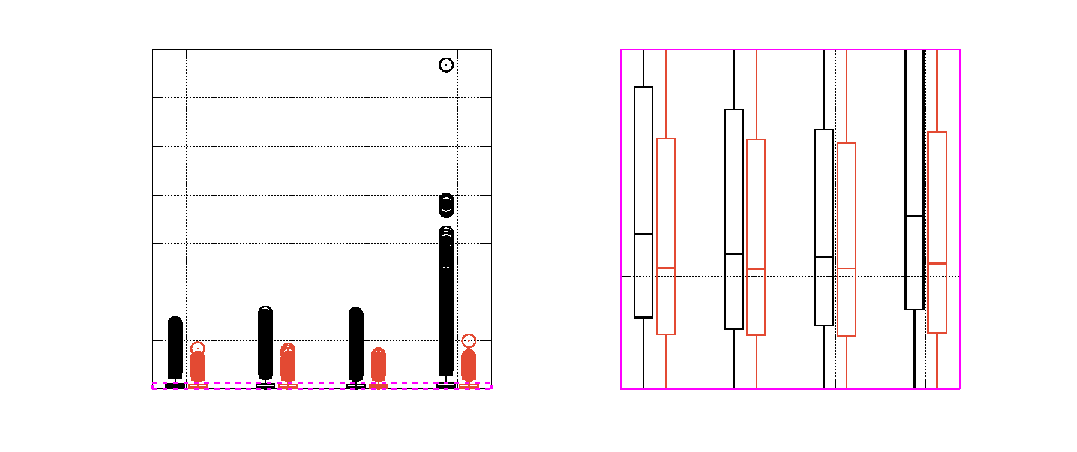
\includegraphics{./figures/parts/appendix/chapters/02/sections/04/corridor_all_orientation_errors_per_selection}}%
    \gplfronttext
  \end{picture}%
\endgroup

    \vspace{0.3cm}
    \caption{Περιβάλλον CORRIDOR}
    \label{}
  \end{subfigure}\\
  \begin{subfigure}{\linewidth}\vspace{0.5cm}
    \hspace{-1.25cm}
    % GNUPLOT: LaTeX picture with Postscript
\begingroup
  \makeatletter
  \providecommand\color[2][]{%
    \GenericError{(gnuplot) \space\space\space\@spaces}{%
      Package color not loaded in conjunction with
      terminal option `colourtext'%
    }{See the gnuplot documentation for explanation.%
    }{Either use 'blacktext' in gnuplot or load the package
      color.sty in LaTeX.}%
    \renewcommand\color[2][]{}%
  }%
  \providecommand\includegraphics[2][]{%
    \GenericError{(gnuplot) \space\space\space\@spaces}{%
      Package graphicx or graphics not loaded%
    }{See the gnuplot documentation for explanation.%
    }{The gnuplot epslatex terminal needs graphicx.sty or graphics.sty.}%
    \renewcommand\includegraphics[2][]{}%
  }%
  \providecommand\rotatebox[2]{#2}%
  \@ifundefined{ifGPcolor}{%
    \newif\ifGPcolor
    \GPcolorfalse
  }{}%
  \@ifundefined{ifGPblacktext}{%
    \newif\ifGPblacktext
    \GPblacktexttrue
  }{}%
  % define a \g@addto@macro without @ in the name:
  \let\gplgaddtomacro\g@addto@macro
  % define empty templates for all commands taking text:
  \gdef\gplfronttext{}%
  \gdef\gplfronttext{}%
  \makeatother
  \ifGPblacktext
    % no textcolor at all
    \def\colorrgb#1{}%
    \def\colorgray#1{}%
  \else
    % gray or color?
    \ifGPcolor
      \def\colorrgb#1{\color[rgb]{#1}}%
      \def\colorgray#1{\color[gray]{#1}}%
      \expandafter\def\csname LTw\endcsname{\color{white}}%
      \expandafter\def\csname LTb\endcsname{\color{black}}%
      \expandafter\def\csname LTa\endcsname{\color{black}}%
      \expandafter\def\csname LT0\endcsname{\color[rgb]{1,0,0}}%
      \expandafter\def\csname LT1\endcsname{\color[rgb]{0,1,0}}%
      \expandafter\def\csname LT2\endcsname{\color[rgb]{0,0,1}}%
      \expandafter\def\csname LT3\endcsname{\color[rgb]{1,0,1}}%
      \expandafter\def\csname LT4\endcsname{\color[rgb]{0,1,1}}%
      \expandafter\def\csname LT5\endcsname{\color[rgb]{1,1,0}}%
      \expandafter\def\csname LT6\endcsname{\color[rgb]{0,0,0}}%
      \expandafter\def\csname LT7\endcsname{\color[rgb]{1,0.3,0}}%
      \expandafter\def\csname LT8\endcsname{\color[rgb]{0.5,0.5,0.5}}%
    \else
      % gray
      \def\colorrgb#1{\color{black}}%
      \def\colorgray#1{\color[gray]{#1}}%
      \expandafter\def\csname LTw\endcsname{\color{white}}%
      \expandafter\def\csname LTb\endcsname{\color{black}}%
      \expandafter\def\csname LTa\endcsname{\color{black}}%
      \expandafter\def\csname LT0\endcsname{\color{black}}%
      \expandafter\def\csname LT1\endcsname{\color{black}}%
      \expandafter\def\csname LT2\endcsname{\color{black}}%
      \expandafter\def\csname LT3\endcsname{\color{black}}%
      \expandafter\def\csname LT4\endcsname{\color{black}}%
      \expandafter\def\csname LT5\endcsname{\color{black}}%
      \expandafter\def\csname LT6\endcsname{\color{black}}%
      \expandafter\def\csname LT7\endcsname{\color{black}}%
      \expandafter\def\csname LT8\endcsname{\color{black}}%
    \fi
  \fi
  \setlength{\unitlength}{0.0500bp}%
  \begin{picture}(10000.00,4000.00)%
    \gplgaddtomacro\gplfronttext{%
      \colorrgb{0.00,0.00,0.00}%
      \put(1168,440){\makebox(0,0)[r]{\strut{}$0.0$}}%
      \colorrgb{0.00,0.00,0.00}%
      \put(1168,766){\makebox(0,0)[r]{\strut{}$0.1$}}%
      \colorrgb{0.00,0.00,0.00}%
      \put(1168,1092){\makebox(0,0)[r]{\strut{}$0.2$}}%
      \colorrgb{0.00,0.00,0.00}%
      \put(1168,1418){\makebox(0,0)[r]{\strut{}$0.3$}}%
      \colorrgb{0.00,0.00,0.00}%
      \put(1168,1744){\makebox(0,0)[r]{\strut{}$0.4$}}%
      \colorrgb{0.00,0.00,0.00}%
      \put(1168,2070){\makebox(0,0)[r]{\strut{}$0.5$}}%
      \colorrgb{0.00,0.00,0.00}%
      \put(1168,2395){\makebox(0,0)[r]{\strut{}$0.6$}}%
      \colorrgb{0.00,0.00,0.00}%
      \put(1168,2395){\makebox(0,0)[r]{\strut{}0.6}}%
      \colorrgb{0.00,0.00,0.00}%
      \put(1168,2721){\makebox(0,0)[r]{\strut{}$0.7$}}%
      \colorrgb{0.00,0.00,0.00}%
      \put(1168,2721){\makebox(0,0)[r]{\strut{}0.7}}%
      \colorrgb{0.00,0.00,0.00}%
      \put(1168,3047){\makebox(0,0)[r]{\strut{}$0.8$}}%
      \colorrgb{0.00,0.00,0.00}%
      \put(1168,3373){\makebox(0,0)[r]{\strut{}$0.9$}}%
      \colorrgb{0.00,0.00,0.00}%
      \put(1168,3699){\makebox(0,0)[r]{\strut{}$1.0$}}%
      \colorrgb{0.00,0.00,0.00}%
      \put(1625,220){\makebox(0,0){\strut{}$100\%$}}%
      \colorrgb{0.00,0.00,0.00}%
      \put(2493,220){\makebox(0,0){\strut{}$>\overline{W}$}}%
      \colorrgb{0.00,0.00,0.00}%
      \put(3361,220){\makebox(0,0){\strut{}$10\%$}}%
      \colorrgb{0.00,0.00,0.00}%
      \put(4229,220){\makebox(0,0){\strut{}top}}%
      \colorrgb{0.00,0.00,0.00}%
      \put(530,2069){\rotatebox{90}{\makebox(0,0){\strut{}$\overline{\|\bm{e}\|_{2,i}}$, $i = \{1,2,\dots,N\}$}}}%
      \colorrgb{0.00,0.00,0.00}%
      \put(2927,-110){\makebox(0,0){\strut{}Μέθοδος επιλογής}}%
      \colorrgb{0.00,0.00,0.00}%
    }%
    \gplgaddtomacro\gplfronttext{%
    }%
    \gplgaddtomacro\gplfronttext{%
      \colorrgb{0.00,0.00,0.00}%
      \put(5663,440){\makebox(0,0)[r]{\strut{}$0.0$}}%
      \colorrgb{0.00,0.00,0.00}%
      \put(5663,1092){\makebox(0,0)[r]{\strut{}$0.002$}}%
      \colorrgb{0.00,0.00,0.00}%
      \put(5663,1744){\makebox(0,0)[r]{\strut{}$0.004$}}%
      \colorrgb{0.00,0.00,0.00}%
      \put(5663,2395){\makebox(0,0)[r]{\strut{}$0.006$}}%
      \colorrgb{0.00,0.00,0.00}%
      \put(5663,3047){\makebox(0,0)[r]{\strut{}$0.008$}}%
      \colorrgb{0.00,0.00,0.00}%
      \put(5663,3699){\makebox(0,0)[r]{\strut{}$0.010$}}%
      \colorrgb{0.00,0.00,0.00}%
      \put(6120,220){\makebox(0,0){\strut{}$100\%$}}%
      \colorrgb{0.00,0.00,0.00}%
      \put(6988,220){\makebox(0,0){\strut{}$>\overline{W}$}}%
      \colorrgb{0.00,0.00,0.00}%
      \put(7856,220){\makebox(0,0){\strut{}$10\%$}}%
      \colorrgb{0.00,0.00,0.00}%
      \put(8724,220){\makebox(0,0){\strut{}top}}%
      \colorrgb{0.00,0.00,0.00}%
      \put(7422,-110){\makebox(0,0){\strut{}Μέθοδος επιλογής}}%
      \colorrgb{0.00,0.00,0.00}%
    }%
    \gplgaddtomacro\gplfronttext{%
    }%
    \gplfronttext
    \put(0,0){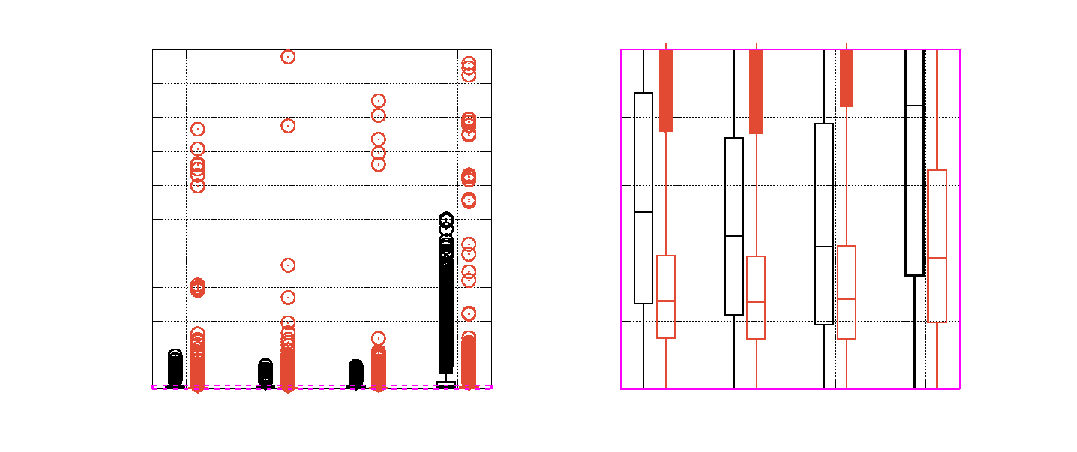
\includegraphics{./figures/parts/appendix/chapters/02/sections/04/warehouse_all_orientation_errors_per_selection}}%
    \gplfronttext
  \end{picture}%
\endgroup

    \vspace{0.3cm}
    \caption{Περιβάλλον WAREHOUSE}
    \label{}
    \end{subfigure}
\caption{\small Η κατανομή του μέσου σφάλματος προσανατολισμού ανά διαδρομή
         πλοήγησης για τον MCL σε ανοιχτό βρόχο (στα αριστερά κάθε
         υποδεικνυόμενης μεθόδου επιλογής, με μαύρο χρώμα) και του σύνθετου
         συστήματος (δεξιά, με κόκκινο), σε $N=100$ προσομοιώσεις, ανάλογα με
         την μέθοδο επιλογής πληθυσμού. Το σύμβολο ``$100\%$" υποδηλώνει τη
         διαμόρφωση του συστήματος όπου όλα τα σωματίδια του συνόλου του
         πληθυσμού επιλέγονται κατά τη διαδικασία εξαγωγής της εκτίμησης της
         στάσης του συστήματος, το σύμβολο ``$>\overline{W}$" υποδηλώνει εκείνη
         της επιλογής των σωματιδίων των οποίων το βάρος είναι μεγαλύτερο από
         το μέσο βάρος του πληθυσμού του φίλτρου, το ``$10\%$" εκείνη που μόνο
         το άνω $10\%$ των βαρύτερων σωματιδίων επιλέγονται, και ``top" τη
         διαμόρφωση όπου επιλέγεται μόνο το σωματίδιο με το μεγαλύτερο βάρος
         μεταξύ όλων των σωματιδίων του πληθυσμού}
\label{fig:02_02_04:selections_orientation_zoomed}
\end{figure}


\begin{figure}
  \vspace{2cm}
  \begin{subfigure}{\linewidth}
  \hspace{-1.25cm}
    % GNUPLOT: LaTeX picture with Postscript
\begingroup
  \makeatletter
  \providecommand\color[2][]{%
    \GenericError{(gnuplot) \space\space\space\@spaces}{%
      Package color not loaded in conjunction with
      terminal option `colourtext'%
    }{See the gnuplot documentation for explanation.%
    }{Either use 'blacktext' in gnuplot or load the package
      color.sty in LaTeX.}%
    \renewcommand\color[2][]{}%
  }%
  \providecommand\includegraphics[2][]{%
    \GenericError{(gnuplot) \space\space\space\@spaces}{%
      Package graphicx or graphics not loaded%
    }{See the gnuplot documentation for explanation.%
    }{The gnuplot epslatex terminal needs graphicx.sty or graphics.sty.}%
    \renewcommand\includegraphics[2][]{}%
  }%
  \providecommand\rotatebox[2]{#2}%
  \@ifundefined{ifGPcolor}{%
    \newif\ifGPcolor
    \GPcolorfalse
  }{}%
  \@ifundefined{ifGPblacktext}{%
    \newif\ifGPblacktext
    \GPblacktexttrue
  }{}%
  % define a \g@addto@macro without @ in the name:
  \let\gplgaddtomacro\g@addto@macro
  % define empty templates for all commands taking text:
  \gdef\gplfronttext{}%
  \gdef\gplfronttext{}%
  \makeatother
  \ifGPblacktext
    % no textcolor at all
    \def\colorrgb#1{}%
    \def\colorgray#1{}%
  \else
    % gray or color?
    \ifGPcolor
      \def\colorrgb#1{\color[rgb]{#1}}%
      \def\colorgray#1{\color[gray]{#1}}%
      \expandafter\def\csname LTw\endcsname{\color{white}}%
      \expandafter\def\csname LTb\endcsname{\color{black}}%
      \expandafter\def\csname LTa\endcsname{\color{black}}%
      \expandafter\def\csname LT0\endcsname{\color[rgb]{1,0,0}}%
      \expandafter\def\csname LT1\endcsname{\color[rgb]{0,1,0}}%
      \expandafter\def\csname LT2\endcsname{\color[rgb]{0,0,1}}%
      \expandafter\def\csname LT3\endcsname{\color[rgb]{1,0,1}}%
      \expandafter\def\csname LT4\endcsname{\color[rgb]{0,1,1}}%
      \expandafter\def\csname LT5\endcsname{\color[rgb]{1,1,0}}%
      \expandafter\def\csname LT6\endcsname{\color[rgb]{0,0,0}}%
      \expandafter\def\csname LT7\endcsname{\color[rgb]{1,0.3,0}}%
      \expandafter\def\csname LT8\endcsname{\color[rgb]{0.5,0.5,0.5}}%
    \else
      % gray
      \def\colorrgb#1{\color{black}}%
      \def\colorgray#1{\color[gray]{#1}}%
      \expandafter\def\csname LTw\endcsname{\color{white}}%
      \expandafter\def\csname LTb\endcsname{\color{black}}%
      \expandafter\def\csname LTa\endcsname{\color{black}}%
      \expandafter\def\csname LT0\endcsname{\color{black}}%
      \expandafter\def\csname LT1\endcsname{\color{black}}%
      \expandafter\def\csname LT2\endcsname{\color{black}}%
      \expandafter\def\csname LT3\endcsname{\color{black}}%
      \expandafter\def\csname LT4\endcsname{\color{black}}%
      \expandafter\def\csname LT5\endcsname{\color{black}}%
      \expandafter\def\csname LT6\endcsname{\color{black}}%
      \expandafter\def\csname LT7\endcsname{\color{black}}%
      \expandafter\def\csname LT8\endcsname{\color{black}}%
    \fi
  \fi
  \setlength{\unitlength}{0.0500bp}%
  \begin{picture}(10000.00,4000.00)%
    \gplgaddtomacro\gplfronttext{%
      \colorrgb{0.00,0.00,0.00}%
      \put(1168,440){\makebox(0,0)[r]{\strut{}$0.0$}}%
      \colorrgb{0.00,0.00,0.00}%
      \put(1168,766){\makebox(0,0)[r]{\strut{}$0.10$}}%
      \colorrgb{0.00,0.00,0.00}%
      \put(1168,1092){\makebox(0,0)[r]{\strut{}$0.20$}}%
      \colorrgb{0.00,0.00,0.00}%
      \put(1168,1418){\makebox(0,0)[r]{\strut{}$0.30$}}%
      \colorrgb{0.00,0.00,0.00}%
      \put(1168,1744){\makebox(0,0)[r]{\strut{}$0.40$}}%
      \colorrgb{0.00,0.00,0.00}%
      \put(1168,2070){\makebox(0,0)[r]{\strut{}$0.50$}}%
      \colorrgb{0.00,0.00,0.00}%
      \put(1168,2395){\makebox(0,0)[r]{\strut{}$0.60$}}%
      \colorrgb{0.00,0.00,0.00}%
      \put(1168,2395){\makebox(0,0)[r]{\strut{}0.6}}%
      \colorrgb{0.00,0.00,0.00}%
      \put(1168,2721){\makebox(0,0)[r]{\strut{}$0.70$}}%
      \colorrgb{0.00,0.00,0.00}%
      \put(1168,2721){\makebox(0,0)[r]{\strut{}0.7}}%
      \colorrgb{0.00,0.00,0.00}%
      \put(1168,3047){\makebox(0,0)[r]{\strut{}$0.80$}}%
      \colorrgb{0.00,0.00,0.00}%
      \put(1168,3373){\makebox(0,0)[r]{\strut{}$0.90$}}%
      \colorrgb{0.00,0.00,0.00}%
      \put(1168,3699){\makebox(0,0)[r]{\strut{}$1.0$}}%
      \colorrgb{0.00,0.00,0.00}%
      \put(1625,220){\makebox(0,0){\strut{}$100\%$}}%
      \colorrgb{0.00,0.00,0.00}%
      \put(2493,220){\makebox(0,0){\strut{}$>\overline{W}$}}%
      \colorrgb{0.00,0.00,0.00}%
      \put(3361,220){\makebox(0,0){\strut{}$10\%$}}%
      \colorrgb{0.00,0.00,0.00}%
      \put(4229,220){\makebox(0,0){\strut{}top}}%
      \colorrgb{0.00,0.00,0.00}%
      \put(398,2069){\rotatebox{90}{\makebox(0,0){\strut{}$\overline{\|e\|_{2,i}}$, $i = \{1,2,\dots,N\}$}}}%
      \colorrgb{0.00,0.00,0.00}%
      \put(2927,-110){\makebox(0,0){\strut{}Μέθοδος επιλογής}}%
      \colorrgb{0.00,0.00,0.00}%
      \put(5000,4129){\makebox(0,0){\strut{}Κατανομή σφαλμάτων εκτίμησης θέσης ανά μέθοδο επιλογής σωματιδίων [m]}}%
    }%
    \gplgaddtomacro\gplfronttext{%
    }%
    \gplgaddtomacro\gplfronttext{%
      \colorrgb{0.00,0.00,0.00}%
      \put(5663,440){\makebox(0,0)[r]{\strut{}$0.0$}}%
      \colorrgb{0.00,0.00,0.00}%
      \put(5663,1255){\makebox(0,0)[r]{\strut{}$0.005$}}%
      \colorrgb{0.00,0.00,0.00}%
      \put(5663,2070){\makebox(0,0)[r]{\strut{}$0.010$}}%
      \colorrgb{0.00,0.00,0.00}%
      \put(5663,2884){\makebox(0,0)[r]{\strut{}$0.015$}}%
      \colorrgb{0.00,0.00,0.00}%
      \put(5663,3699){\makebox(0,0)[r]{\strut{}$0.020$}}%
      \colorrgb{0.00,0.00,0.00}%
      \put(6120,220){\makebox(0,0){\strut{}$100\%$}}%
      \colorrgb{0.00,0.00,0.00}%
      \put(6988,220){\makebox(0,0){\strut{}$>\overline{W}$}}%
      \colorrgb{0.00,0.00,0.00}%
      \put(7856,220){\makebox(0,0){\strut{}$10\%$}}%
      \colorrgb{0.00,0.00,0.00}%
      \put(8724,220){\makebox(0,0){\strut{}top}}%
      \colorrgb{0.00,0.00,0.00}%
      \put(4761,2069){\rotatebox{90}{\makebox(0,0){\strut{}$\overline{\|e\|_{2,i}}$, $i = \{1,2,\dots,N\}$}}}%
      \colorrgb{0.00,0.00,0.00}%
      \put(7422,-110){\makebox(0,0){\strut{}Μέθοδος επιλογής}}%
      \colorrgb{0.00,0.00,0.00}%
    }%
    \gplgaddtomacro\gplfronttext{%
    }%
    \gplfronttext
    \put(0,0){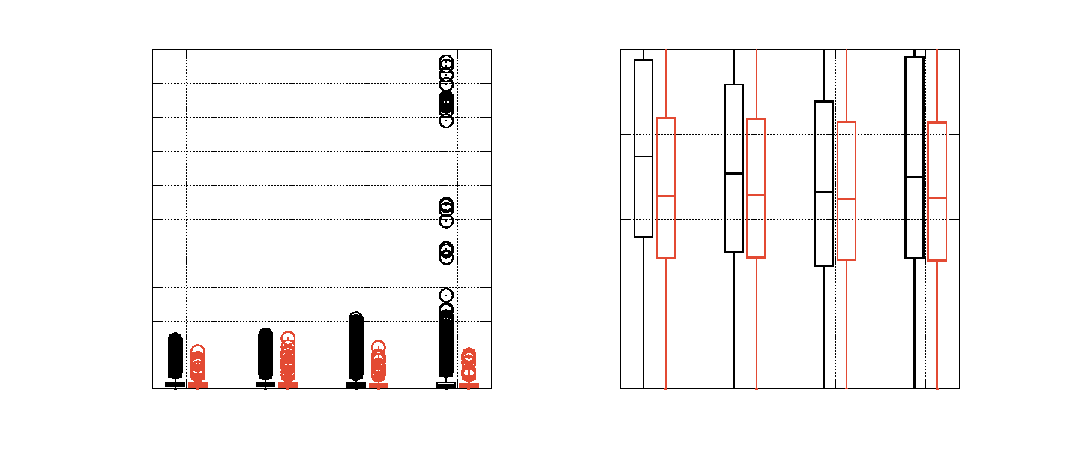
\includegraphics{./figures/parts/appendix/chapters/02/sections/04/corridor_all_position_errors_per_selection}}%
    \gplfronttext
  \end{picture}%
\endgroup

    \vspace{0.3cm}
    \caption{Περιβάλλον CORRIDOR}
    \label{}
  \end{subfigure}\\
  \begin{subfigure}{\linewidth}\vspace{0.5cm}
    \hspace{-1.25cm}
    % GNUPLOT: LaTeX picture with Postscript
\begingroup
  \makeatletter
  \providecommand\color[2][]{%
    \GenericError{(gnuplot) \space\space\space\@spaces}{%
      Package color not loaded in conjunction with
      terminal option `colourtext'%
    }{See the gnuplot documentation for explanation.%
    }{Either use 'blacktext' in gnuplot or load the package
      color.sty in LaTeX.}%
    \renewcommand\color[2][]{}%
  }%
  \providecommand\includegraphics[2][]{%
    \GenericError{(gnuplot) \space\space\space\@spaces}{%
      Package graphicx or graphics not loaded%
    }{See the gnuplot documentation for explanation.%
    }{The gnuplot epslatex terminal needs graphicx.sty or graphics.sty.}%
    \renewcommand\includegraphics[2][]{}%
  }%
  \providecommand\rotatebox[2]{#2}%
  \@ifundefined{ifGPcolor}{%
    \newif\ifGPcolor
    \GPcolorfalse
  }{}%
  \@ifundefined{ifGPblacktext}{%
    \newif\ifGPblacktext
    \GPblacktexttrue
  }{}%
  % define a \g@addto@macro without @ in the name:
  \let\gplgaddtomacro\g@addto@macro
  % define empty templates for all commands taking text:
  \gdef\gplfronttext{}%
  \gdef\gplfronttext{}%
  \makeatother
  \ifGPblacktext
    % no textcolor at all
    \def\colorrgb#1{}%
    \def\colorgray#1{}%
  \else
    % gray or color?
    \ifGPcolor
      \def\colorrgb#1{\color[rgb]{#1}}%
      \def\colorgray#1{\color[gray]{#1}}%
      \expandafter\def\csname LTw\endcsname{\color{white}}%
      \expandafter\def\csname LTb\endcsname{\color{black}}%
      \expandafter\def\csname LTa\endcsname{\color{black}}%
      \expandafter\def\csname LT0\endcsname{\color[rgb]{1,0,0}}%
      \expandafter\def\csname LT1\endcsname{\color[rgb]{0,1,0}}%
      \expandafter\def\csname LT2\endcsname{\color[rgb]{0,0,1}}%
      \expandafter\def\csname LT3\endcsname{\color[rgb]{1,0,1}}%
      \expandafter\def\csname LT4\endcsname{\color[rgb]{0,1,1}}%
      \expandafter\def\csname LT5\endcsname{\color[rgb]{1,1,0}}%
      \expandafter\def\csname LT6\endcsname{\color[rgb]{0,0,0}}%
      \expandafter\def\csname LT7\endcsname{\color[rgb]{1,0.3,0}}%
      \expandafter\def\csname LT8\endcsname{\color[rgb]{0.5,0.5,0.5}}%
    \else
      % gray
      \def\colorrgb#1{\color{black}}%
      \def\colorgray#1{\color[gray]{#1}}%
      \expandafter\def\csname LTw\endcsname{\color{white}}%
      \expandafter\def\csname LTb\endcsname{\color{black}}%
      \expandafter\def\csname LTa\endcsname{\color{black}}%
      \expandafter\def\csname LT0\endcsname{\color{black}}%
      \expandafter\def\csname LT1\endcsname{\color{black}}%
      \expandafter\def\csname LT2\endcsname{\color{black}}%
      \expandafter\def\csname LT3\endcsname{\color{black}}%
      \expandafter\def\csname LT4\endcsname{\color{black}}%
      \expandafter\def\csname LT5\endcsname{\color{black}}%
      \expandafter\def\csname LT6\endcsname{\color{black}}%
      \expandafter\def\csname LT7\endcsname{\color{black}}%
      \expandafter\def\csname LT8\endcsname{\color{black}}%
    \fi
  \fi
  \setlength{\unitlength}{0.0500bp}%
  \begin{picture}(10000.00,4000.00)%
    \gplgaddtomacro\gplfronttext{%
      \colorrgb{0.00,0.00,0.00}%
      \put(1168,440){\makebox(0,0)[r]{\strut{}$0.0$}}%
      \colorrgb{0.00,0.00,0.00}%
      \put(1168,1092){\makebox(0,0)[r]{\strut{}$1.0$}}%
      \colorrgb{0.00,0.00,0.00}%
      \put(1168,1744){\makebox(0,0)[r]{\strut{}$2.0$}}%
      \colorrgb{0.00,0.00,0.00}%
      \put(1168,2395){\makebox(0,0)[r]{\strut{}$3.0$}}%
      \colorrgb{0.00,0.00,0.00}%
      \put(1168,3047){\makebox(0,0)[r]{\strut{}$4.0$}}%
      \colorrgb{0.00,0.00,0.00}%
      \put(1168,3699){\makebox(0,0)[r]{\strut{}$5.0$}}%
      \colorrgb{0.00,0.00,0.00}%
      \put(1625,220){\makebox(0,0){\strut{}$100\%$}}%
      \colorrgb{0.00,0.00,0.00}%
      \put(2493,220){\makebox(0,0){\strut{}$>\overline{W}$}}%
      \colorrgb{0.00,0.00,0.00}%
      \put(3361,220){\makebox(0,0){\strut{}$10\%$}}%
      \colorrgb{0.00,0.00,0.00}%
      \put(4229,220){\makebox(0,0){\strut{}top}}%
      \colorrgb{0.00,0.00,0.00}%
      \put(530,2069){\rotatebox{90}{\makebox(0,0){\strut{}$\overline{\|e\|_{2,i}}$, $i = \{1,2,\dots,N\}$}}}%
      \colorrgb{0.00,0.00,0.00}%
      \put(2927,-110){\makebox(0,0){\strut{}Μέθοδος επιλογής}}%
      \colorrgb{0.00,0.00,0.00}%
    }%
    \gplgaddtomacro\gplfronttext{%
    }%
    \gplgaddtomacro\gplfronttext{%
      \colorrgb{0.00,0.00,0.00}%
      \put(5663,440){\makebox(0,0)[r]{\strut{}$0.0$}}%
      \colorrgb{0.00,0.00,0.00}%
      \put(5663,1092){\makebox(0,0)[r]{\strut{}$0.02$}}%
      \colorrgb{0.00,0.00,0.00}%
      \put(5663,1744){\makebox(0,0)[r]{\strut{}$0.04$}}%
      \colorrgb{0.00,0.00,0.00}%
      \put(5663,2395){\makebox(0,0)[r]{\strut{}$0.06$}}%
      \colorrgb{0.00,0.00,0.00}%
      \put(5663,3047){\makebox(0,0)[r]{\strut{}$0.08$}}%
      \colorrgb{0.00,0.00,0.00}%
      \put(5663,3699){\makebox(0,0)[r]{\strut{}$0.10$}}%
      \colorrgb{0.00,0.00,0.00}%
      \put(6120,220){\makebox(0,0){\strut{}$100\%$}}%
      \colorrgb{0.00,0.00,0.00}%
      \put(6988,220){\makebox(0,0){\strut{}$>\overline{W}$}}%
      \colorrgb{0.00,0.00,0.00}%
      \put(7856,220){\makebox(0,0){\strut{}$10\%$}}%
      \colorrgb{0.00,0.00,0.00}%
      \put(8724,220){\makebox(0,0){\strut{}top}}%
      \colorrgb{0.00,0.00,0.00}%
      \put(4893,2069){\rotatebox{90}{\makebox(0,0){\strut{}$\overline{\|e\|_{2,i}}$, $i = \{1,2,\dots,N\}$}}}%
      \colorrgb{0.00,0.00,0.00}%
      \put(7422,-110){\makebox(0,0){\strut{}Μέθοδος επιλογής}}%
      \colorrgb{0.00,0.00,0.00}%
    }%
    \gplgaddtomacro\gplfronttext{%
    }%
    \gplfronttext
    \put(0,0){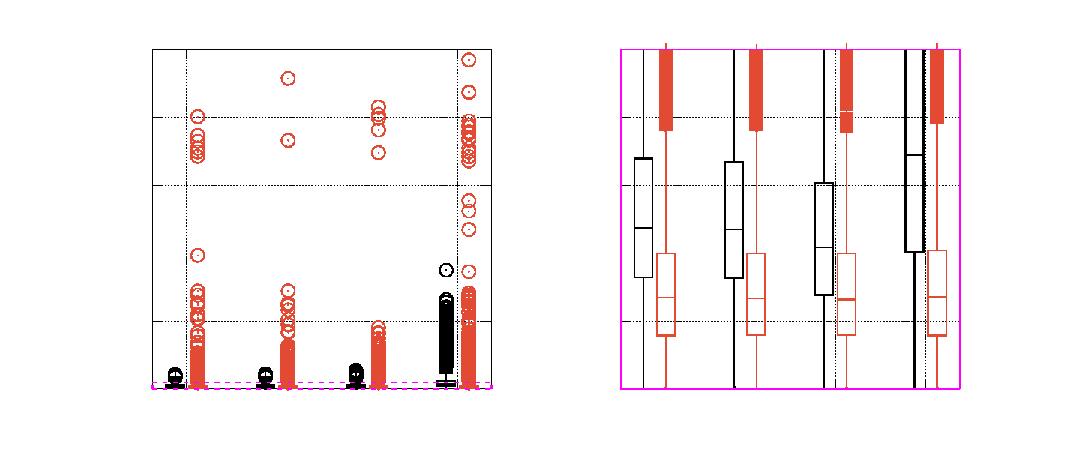
\includegraphics{./figures/parts/appendix/chapters/02/sections/04/warehouse_all_position_errors_per_selection}}%
    \gplfronttext
  \end{picture}%
\endgroup

    \vspace{0.3cm}
    \caption{Περιβάλλον WAREHOUSE}
    \label{}
    \end{subfigure}
\caption{\small Η κατανομή του μέσου σφάλματος θέσης ανά διαδρομή πλοήγησης
         για τον MCL σε ανοιχτό βρόχο (στα αριστερά κάθε υποδεικνυόμενης
         μεθόδου επιλογής, με μαύρο χρώμα) και του σύνθετου συστήματος (δεξιά,
         με κόκκινο), σε $N=100$ προσομοιώσεις, ανάλογα με την μέθοδο επιλογής
         πληθυσμού. Το σύμβολο ``$100\%$" υποδηλώνει τη διαμόρφωση του
         συστήματος όπου όλα τα σωματίδια του συνόλου του πληθυσμού επιλέγονται
         κατά τη διαδικασία εξαγωγής της εκτίμησης της στάσης του συστήματος,
         το σύμβολο ``$>\overline{W}$" υποδηλώνει εκείνη της επιλογής των
         σωματιδίων των οποίων το βάρος είναι μεγαλύτερο από το μέσο βάρος του
         πληθυσμού του φίλτρου, το ``$10\%$" εκείνη που μόνο το άνω $10\%$ των
         βαρύτερων σωματιδίων επιλέγονται, και ``top" τη διαμόρφωση όπου
         επιλέγεται μόνο το σωματίδιο με το μεγαλύτερο βάρος μεταξύ όλων των
         σωματιδίων του πληθυσμού}
\label{fig:02_02_04:selections_position_zoomed}
\end{figure}
